% \chapter{Project Prototype}

% This section presents the prototype implementation of the proposed system, focusing on how the Adaptive AUTOSAR architecture is instantiated and evaluated in practice. The prototype is designed to demonstrate the feasibility of integrating perception, communication, and warning functionalities within a service-oriented automotive software framework.

% \begin{figure}[H]
%     \centering
%     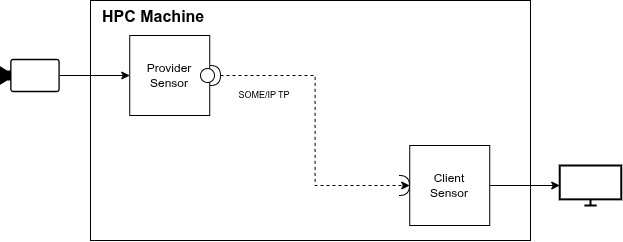
\includegraphics[width=0.75\textwidth]{Images/chapter4/archDesign.png}
%     \vspace{0.5cm}
%     \caption{The architecture design of prototype project}
%     \label{fig:archDesign_project}
% \end{figure}

% Figure~\ref{fig:archDesign_project} illustrates the overall architecture of the prototype system deployed on a High-Performance Computing (HPC) machine. The design follows the Adaptive AUTOSAR methodology, in which software functionalities are decomposed into independent applications that communicate through well-defined service interfaces. In the proposed prototype, the system is organized around two main applications, namely the Provider Sensor and the Client Sensor, which interact through SOME/IP with transport protocol (SOME/IP-TP).

% The Provider Sensor is responsible for collecting, decoding, and processing sensor-related input data, as well as providing processed information to other applications in the system. It acts as a data provider within the service-oriented architecture, exposing its services to subscribed clients. The Client Sensor consumes the provided data, performs perception and decision-related tasks, and generates user-facing outputs such as warnings or visualization results. This clear separation of responsibilities improves modularity and reflects typical ADAS software design principles.

% The prototype focuses on validating both functional correctness and system integration aspects rather than achieving production-level optimization. All applications are executed within a controlled Adaptive AUTOSAR runtime environment, enabling evaluation of inter-application communication, execution flow, and end-to-end behavior. The following subsections describe the implementation details of each component and present the experimental results obtained from the prototype evaluation.

% \chapter{Provider Sensor}
% 

% \chapter{Flow Chart}
% \begin{figure}[H]
% \centering
% \begin{tikzpicture}[
%     node distance=1.5cm,
%     every node/.style={font=\small},
%     startstop/.style={
%         rectangle, rounded corners,
%         minimum width=3.6cm,
%         minimum height=0.9cm,
%         draw, align=center
%     },
%     process/.style={
%         rectangle,
%         minimum width=4.4cm,
%         minimum height=0.9cm,
%         draw, align=center
%     },
%     decision/.style={
%         diamond,
%         aspect=2.8,
%         minimum width=2.6cm,
%         minimum height=0.85cm,
%         inner sep=1.5pt,
%         draw, align=center
%     },
%     arrow/.style={->, thick},
% ]

% % ===== Nodes =====
% \node (start) [startstop] {Application Start};

% \node (init) [process, below of=start] {Initialize ProviderSensor};

% \node (tflite) [process, below of=init] {Initialize TFLite Model};

% \node (checkinit) [decision, below of=tflite, yshift=-0.5cm]
% {Initialization Successful};

% \node (terminate) [startstop, right=3.8cm of checkinit]
% {Terminate Application};

% \node (startport) [process, below of=checkinit, yshift=-0.4cm]
% {Start Sensorv2 Port};

% \node (run) [process, below of=startport]
% {Run Application Thread};

% \node (caminit) [process, below of=run]
% {Open Camera Device};

% \node (camcheck) [decision, below of=caminit, yshift=-0.5cm]
% {Camera Opened};

% \node (cont) [startstop, below of=camcheck, yshift=-0.4cm]
% {Enter Main Processing Loop};

% % ===== Arrows =====
% \draw [arrow] (start) -- (init);
% \draw [arrow] (init) -- (tflite);
% \draw [arrow] (tflite) -- (checkinit);

% \draw [arrow] (checkinit) -- node[right]{Yes} (startport);
% \draw [arrow] (checkinit.east) -- node[above]{No} (terminate.west);

% \draw [arrow] (startport) -- (run);
% \draw [arrow] (run) -- (caminit);
% \draw [arrow] (caminit) -- (camcheck);

% \draw [arrow] (camcheck) -- node[right]{Yes} (cont);
% \draw [arrow]
%     (camcheck.east)
%     -| node[near start, above]{No}
%     (terminate.south);

% \end{tikzpicture}
% \vspace{0.5cm}
% \caption{Initialization Flow of the ProviderSensor Adaptive Application}
% \label{fig:providersensor_init}
% \end{figure}

% \begin{figure}[H]
% \centering
% \begin{tikzpicture}[
%     node distance=1.4cm,
%     every node/.style={font=\small},
%     startstop/.style={
%         rectangle, rounded corners,
%         minimum width=3.6cm,
%         minimum height=0.9cm,
%         draw, align=center
%     },
%     process/.style={
%         rectangle,
%         minimum width=4.6cm,
%         minimum height=0.9cm,
%         draw, align=center
%     },
%     decision/.style={
%         diamond,
%         aspect=2.6,
%         minimum width=3.2cm,
%         minimum height=1.0cm,
%         inner sep=1.5pt,
%         draw, align=center
%     },
%     arrow/.style={->, thick}
% ]

% % ===== Nodes =====
% \node (loop) [startstop] {Main Processing Loop};

% \node (capture) [process, below of=loop]
% {Capture Camera Frame};

% \node (frameok) [decision, below of=capture]
% {Frame Valid};

% \node (infer) [process, below of=frameok, yshift=-0.4cm]
% {YOLO TFLite Inference};

% \node (post) [process, below of=infer]
% {Post Processing\\ Confidence Filter and NMS};

% \node (drawbox) [process, below of=post]
% {Draw Bounding Boxes};

% \node (encode) [process, below of=drawbox]
% {Encode Frame to JPEG};

% \node (send) [process, below of=encode]
% {Send Data via Sensorv2 Port};

% \node (sleep) [process, below of=send]
% {Sleep to Control Frame Rate};

% % ===== Arrows =====
% \draw [arrow] (loop) -- (capture);
% \draw [arrow] (capture) -- (frameok);

% % Decision: Frame Valid
% \draw [arrow] (frameok) -- node[right]{Yes} (infer);
% \draw [arrow]
%     (frameok.east) -- ++(2.2cm,0)
%     |- node[near start, above]{No} (capture.east);

% % Main pipeline
% \draw [arrow] (infer) -- (post);
% \draw [arrow] (post) -- (drawbox);
% \draw [arrow] (drawbox) -- (encode);
% \draw [arrow] (encode) -- (send);
% \draw [arrow] (send) -- (sleep);

% % Loop back
% \draw [arrow]
%     (sleep.west) -- ++(-2.6cm,0)
%     |- (loop.west);

% \end{tikzpicture}
% \vspace{0.5cm}
% \caption{Runtime Processing Loop of the ProviderSensor Application}
% \label{fig:providersensor_runtime}
% \end{figure}

% The process begins with the application startup, followed immediately by the initialization of the \texttt{ProviderSensor} component and the TensorFlow Lite (TFLite) model. The system then verifies if the initialization was successful. If the initialization fails, the application terminates immediately. Upon success, the system starts the \texttt{Sensorv2} communication port and launches the application thread. The flow proceeds to open the camera device. A check is performed to confirm if the camera opened successfully; if not, the application terminates. If the camera is successfully accessed, the system transitions into the main processing loop.

% Once inside the main processing loop, the system continuously captures camera frames. For each iteration, it verifies if the captured frame is valid. If the frame is invalid, the loop restarts. If valid, the system performs inference using the YOLO TFLite model, followed by post-processing steps which include applying a confidence filter and Non-Maximum Suppression (NMS) to refine detections. The system then draws bounding boxes around detected objects and encodes the frame into JPEG format. This processed data is sent via the \texttt{Sensorv2} port. Finally, the loop includes a sleep interval to control the frame rate before repeating the process.




% \chapter{Flow Chart}
\begin{figure}[H]
\centering
\begin{tikzpicture}[
    scale=0.9, transform shape,
    node distance=1.5cm,
    every node/.style={font=\small},
    startstop/.style={
        rectangle, rounded corners,
        minimum width=3.6cm,
        minimum height=0.9cm,
        draw, align=center
    },
    process/.style={
        rectangle,
        minimum width=4.4cm,
        minimum height=0.9cm,
        draw, align=center
    },
    io/.style={
        trapezium, trapezium left angle=70, trapezium right angle=110,
        minimum width=4.0cm, minimum height=0.9cm,
        inner xsep=0.5cm,
        draw, align=center
    },
    decision/.style={
        diamond,
        aspect=2.8,
        minimum width=2.6cm,
        minimum height=0.85cm,
        inner sep=1.5pt,
        draw, align=center
    },
    arrow/.style={->, thick},
]

% ===== Nodes =====
\node (start) [startstop] {Application Start};

\node (init) [process, below of=start] {Initialize Provider Application};

\node (caminit) [process, below of=init] {Open UART (GPS) \& USB (Webcam)};

\node (checkinit) [decision, below of=caminit, yshift=-0.5cm]
{Devices Opened?};

\node (terminate) [startstop, right=3.8cm of checkinit]
{Terminate Application};

\node (startdds) [process, below of=checkinit, yshift=-0.4cm]
{Initialize DDS Publisher\\Service: \texttt{Sensor}, ID: \texttt{100}};

\node (loop) [startstop, below of=startdds]
{Main Processing Loop};

\node (capture) [io, below of=loop]
{1. Data Acquisition (GPS \& Frame)};

\node (yolo) [process, below of=capture]
{2a. YOLO Traffic Light Detection};

% Multi-thread fork (One thread per Direction)
\node (fork) [rectangle, fill=black, inner sep=0pt, minimum width=8.5cm, minimum height=0.15cm, below of=yolo, yshift=-0.2cm] {};

\node (t1) [process, minimum width=3.6cm, align=center, below of=fork, xshift=-2.8cm, yshift=-0.4cm]
{\textbf{Thread 1 (e.g., Left)}\\Extract ROI\\HSV Color Pipeline\\Timer Detection};

\node (tn) [process, minimum width=3.6cm, align=center, below of=fork, xshift=2.8cm, yshift=-0.4cm]
{\textbf{Thread 3 (e.g., Straight)}\\Extract ROI\\HSV Color Pipeline\\Timer Detection};

\node (dots) [below of=fork, yshift=-1.9cm] {\Large $\dots$};

% Multi-thread join
\node (join) [rectangle, fill=black, inner sep=0pt, minimum width=8.5cm, minimum height=0.15cm, below of=t1, xshift=2.8cm, yshift=-0.8cm] {};

\node (pack) [process, below of=join, yshift=0.3cm]
{3. Pack \texttt{GpsJpegWireHeader} + JPEG};

\node (publish) [io, below of=pack]
{4. Publish \texttt{imageDataEvent}\\Topic: \texttt{imageData}};

% ===== Arrows =====
\draw [arrow] (start) -- (init);
\draw [arrow] (init) -- (caminit);
\draw [arrow] (caminit) -- (checkinit);

\draw [arrow] (checkinit) -- node[right]{Yes} (startdds);
\draw [arrow] (checkinit.east) -- node[above]{No} (terminate.west);

\draw [arrow] (startdds) -- (loop);
\draw [arrow] (loop) -- (capture);
\draw [arrow] (capture) -- (yolo);

\draw [arrow] (yolo) -- (fork);
\draw [arrow] (t1.north |- fork.south) -- (t1.north);
\draw [arrow] (tn.north |- fork.south) -- (tn.north);

\draw [arrow] (t1.south) -- (t1.south |- join.north);
\draw [arrow] (tn.south) -- (tn.south |- join.north);
\draw [arrow] (join.south) -- (pack.north);

\draw [arrow] (pack) -- (publish);

% Loop back
\draw [arrow]
    (publish.west) -- ++(-3.8cm,0)
    |- (loop.west);

\end{tikzpicture}
\vspace{0.5cm}
\caption{Processing Flow of the Provider Application}
\label{fig:provider_flow}
\end{figure}

The application initiates the Provider component by acquiring access to the necessary external peripherals: the GPS module via UART (\texttt{/dev/ttyAMA0}) and the external webcam via USB 2.0 (UVC). Upon successful hardware initialization, the application establishes the DDS Publisher node configured for the \texttt{Sensor} service (instance-id~\texttt{100}, Domain Id~\texttt{0}) using the \texttt{CycloneDDS-CXX} stack over UDP. Failure at either the hardware or network initialization stage results in an immediate application termination to ensure system safety.

Once the setup is complete, the execution enters the main processing loop where data acquisition and perception tasks operate continuously. The pipeline captures a raw video frame from the webcam simultaneously with the reading of GPS position data. The raw frame is passed to the YOLO-based Traffic Light Detection module to infer initial bounding boxes. To meet real-time constraints, the subsequent processing stages are parallelized. The algorithm selects the highest-confidence bounding box for each distinct traffic light direction (Left, Right, Straight) and dispatches a dedicated worker thread for each direction. The concurrent operations within these threads are detailed in Figure~\ref{fig:thread_flow}.

\begin{figure}[H]
\centering
\begin{tikzpicture}[
    scale=0.9, transform shape,
    node distance=1.4cm,
    every node/.style={font=\small},
    startstop/.style={
        rectangle, rounded corners,
        minimum width=3.6cm,
        minimum height=0.9cm,
        draw, align=center
    },
    process/.style={
        rectangle,
        minimum width=4.8cm,
        minimum height=0.9cm,
        draw, align=center
    },
    decision/.style={
        diamond,
        aspect=2.8,
        minimum width=3.0cm,
        minimum height=1.0cm,
        inner sep=1.5pt,
        draw, align=center
    },
    arrow/.style={->, thick},
]

% Nodes
\node (start) [startstop] {Thread Start (dirWorker)};

\node (extract_tl) [process, below of=start] {Extract Traffic Light ROI\\on Original High-Res Image};

\node (hsv) [process, below of=extract_tl] {HSV Color Classification};

\node (check_timer) [decision, below of=hsv, yshift=-0.5cm] {Timer Boxes\\Detected?};

\node (find_nearest) [process, below of=check_timer, yshift=-0.5cm] {Find Nearest Timer Box\\(Distance Calculation)};

\node (check_nearest) [decision, below of=find_nearest, yshift=-0.5cm] {Valid Timer\\Box Found?};

\node (extract_timer) [process, below of=check_nearest, yshift=-0.5cm] {Extract Timer ROI\\on Original High-Res Image};

\node (ocr) [process, below of=extract_timer] {Lightweight OCR Model\\(Digit Recognition)};

\node (end) [startstop, right=3.5cm of check_nearest] {Return Direction\\Result};

% Arrows
\draw [arrow] (start) -- (extract_tl);
\draw [arrow] (extract_tl) -- (hsv);
\draw [arrow] (hsv) -- (check_timer);

\draw [arrow] (check_timer) -- node[right]{Yes} (find_nearest);
\draw [arrow] (check_timer.east) -| node[near start, above]{No} (end.north);

\draw [arrow] (find_nearest) -- (check_nearest);
\draw [arrow] (check_nearest) -- node[above]{No} (end.west);
\draw [arrow] (check_nearest) -- node[right]{Yes} (extract_timer);

\draw [arrow] (extract_timer) -- (ocr);
\draw [arrow] (ocr.east) -| (end.south);

\end{tikzpicture}
\vspace{0.5cm}
\caption{Parallel Thread Pipeline for each Direction (dirWorker)}
\label{fig:thread_flow}
\end{figure}

Within each direction's worker thread (\texttt{dirWorker}), the pipeline maps the low-resolution YOLO bounding box back to the original high-resolution frame to extract a precise Region of Interest (ROI). This ROI undergoes an HSV color space transformation to robustly classify the current signal state. Concurrently, the thread identifies any timer boxes detected in the main frame. By calculating geometric distances, the algorithm pairs the nearest valid timer box with the corresponding traffic light direction. If a match is found, the timer's ROI is extracted from the high-resolution frame and passed through a lightweight OCR model to recognize the remaining countdown digits.

Upon the completion of all parallel threads, the main thread synchronizes the multi-directional results. The annotated frame is then JPEG-encoded and serialized alongside a 24-byte \texttt{GpsJpegWireHeader}. This custom header encapsulates the metadata, including the magic value, protocol version, \texttt{in\_range} flag, \texttt{node\_id}, \texttt{dist\_m}, and the payload length (\texttt{jpeg\_len}). Finally, the combined byte sequence is written into the \texttt{imageData} payload of the \texttt{dds::sensorCam::imageDataEventType} structure and published over the DDS network to any subscribed clients.


% \chapter{Client Sensor}
% % \chapter{Flow Chart}

% \begin{figure}[H]
% \centering
% \begin{tikzpicture}[
%     node distance=1.4cm,
%     every node/.style={font=\small},
%     startstop/.style={
%         rectangle, rounded corners,
%         minimum width=3.8cm,
%         minimum height=0.9cm,
%         draw, align=center
%     },
%     process/.style={
%         rectangle,
%         minimum width=4.8cm,
%         minimum height=0.9cm,
%         draw, align=center
%     },
%     decision/.style={
%         diamond,
%         aspect=2.6,
%         minimum width=3.6cm,
%         minimum height=1.1cm,
%         inner sep=1.5pt,
%         draw, align=center
%     },
%     arrow/.style={->, thick}
% ]

% % ===== Nodes =====
% \node (start) [startstop] {Application Start};

% \node (init) [process, below of=start]
% {Initialize ClientSensor};

% \node (register) [process, below of=init]
% {Register Sensorv2\\ Event Handler};

% \node (startport) [process, below of=register]
% {Start Sensorv2 Port};

% \node (wait) [process, below of=startport]
% {Wait for Incoming Data Event};

% \node (dataok) [decision, below of=wait]
% {Data Received};

% \node (decode) [process, below of=dataok, yshift=-0.4cm]
% {Decode JPEG Data};

% \node (decodeok) [decision, below of=decode]
% {Decode Successful};

% \node (save) [process, below of=decodeok, yshift=-0.4cm]
% {Save Image to File};

% \node (saveok) [decision, below of=save]
% {Save Successful};

% \node (logerr) [process, right=4.6cm of decodeok]
% {Log Error};

% % ===== Main Flow =====
% \draw [arrow] (start) -- (init);
% \draw [arrow] (init) -- (register);
% \draw [arrow] (register) -- (startport);
% \draw [arrow] (startport) -- (wait);
% \draw [arrow] (wait) -- (dataok);

% % Data received decision
% \draw [arrow] (dataok) -- node[right]{Yes} (decode);
% \draw [arrow] (dataok.west) -- ++(-1cm,0) |- node[near start, above]{No} (wait.west);

% % Decode path
% \draw [arrow] (decode) -- (decodeok);

% \draw [arrow] (decodeok) -- node[right]{Yes} (save);
% \draw [arrow] (decodeok.east) -- node[near start, above]{No} (logerr.west);

% % Save decision
% \draw [arrow] (save) -- (saveok);

% \draw [arrow]
%     (saveok.west)
%     -- ++(-1.6cm,0)
%     |- node[near start, above]{Yes}
%     (wait.west);
    
% \draw [arrow] (saveok.east) -| node[near start, above]{No} (logerr.south);

% % Error loop back
% \draw [arrow] (logerr.north) |- (wait.east);


% \end{tikzpicture}

% \vspace{0.5cm}
% \caption{ClientSensor Data Reception and Processing Flow}
% \label{fig:clientsensor_flow}
% \end{figure}

% Data Reception and Processing Flow The Client Sensor workflow starts with the application launch and the initialization of the \texttt{ClientSensor} unit. The system registers the \texttt{Sensorv2} event handler and starts the \texttt{Sensorv2} port to enable communication. It then enters a standby state to wait for incoming data events. When data is received, the system attempts to decode the incoming JPEG data. A decision block checks if the decoding was successful; if not, an error is logged. If decoding succeeds, the system proceeds to save the image to a file. A final check confirms if the file save was successful. If the save operation fails, an error is logged; otherwise, the data handling for that event is considered complete.


% \subsection{Flow Chart}

\begin{figure}[H]
\centering
\begin{tikzpicture}[
    node distance=1.4cm,
    every node/.style={font=\small},
    startstop/.style={
        rectangle, rounded corners,
        minimum width=3.8cm,
        minimum height=0.9cm,
        draw, align=center
    },
    process/.style={
        rectangle,
        minimum width=4.8cm,
        minimum height=0.9cm,
        draw, align=center
    },
    decision/.style={
        diamond,
        aspect=2.6,
        minimum width=3.6cm,
        minimum height=1.1cm,
        inner sep=1.5pt,
        draw, align=center
    },
    arrow/.style={->, thick}
]

% ===== Nodes =====
\node (start) [startstop] {Application Start};

\node (init) [process, below of=start]
{Initialize Client Application};

\node (sub) [process, below of=init]
{1. Subscribe \texttt{imageDataEvent}\\Topic: \texttt{imageData}};

\node (wait) [process, below of=sub]
{Wait for \texttt{imageDataEvent}};

\node (dataok) [decision, below of=wait]
{Event Received};

\node (parse) [process, below of=dataok, yshift=-0.4cm]
{2. Parse \texttt{GpsJpegWireHeader} + JPEG};

\node (tcp) [process, below of=parse]
{3. TCP Client\\\texttt{127.0.0.1:8888}};

\node (sendok) [decision, below of=tcp, yshift=-0.4cm]
{Transmission Successful};

\node (out) [process, below of=sendok, yshift=-0.4cm]
{4. Output to External Display};

\node (logerr) [process, right=4.6cm of dataok]
{Log Error};

% ===== Main Flow =====
\draw [arrow] (start) -- (init);
\draw [arrow] (init) -- (sub);
\draw [arrow] (sub) -- (wait);
\draw [arrow] (wait) -- (dataok);

% Data received decision
\draw [arrow] (dataok) -- node[right]{Yes} (parse);
\draw [arrow] (dataok.west) -- ++(-1cm,0) |- node[near start, above]{No} (wait.west);

% Decode path
\draw [arrow] (parse) -- (tcp);
\draw [arrow] (tcp) -- (sendok);

\draw [arrow] (sendok) -- node[right]{Yes} (out);
\draw [arrow] (sendok.east) -| node[near start, above]{No} (logerr.south);

% Loop back
\draw [arrow]
    (out.west)
    -- ++(-1.6cm,0)
    |-
    (wait.west);
    
% Error loop back
\draw [arrow] (logerr.north) |- (wait.east);

\end{tikzpicture}

\vspace{0.5cm}
\caption{Client Data Reception and Processing Flow}
\label{fig:client_flow}
\end{figure}

Upon startup, the Client application initializes its DDS Subscriber node. It registers a listener for the \texttt{imageDataEvent} on the \texttt{imageData} topic, targeting the \texttt{Sensor} service. The application is configured to discover any available provider (instance-id~\texttt{ANY}) operating on Domain Id~\texttt{0}. Once the DDS entities are established via the \texttt{CycloneDDS-CXX} middleware, the subscriber thread blocks and waits for incoming \texttt{dds::sensorCam::imageDataEventType} messages.

Upon receiving an event, the application extracts the \texttt{imageData} payload and decodes its byte structure. The parser reads the initial 24 bytes to reconstruct the \texttt{GpsJpegWireHeader}, extracting vital metadata such as the \texttt{in\_range} flag, \texttt{node\_id}, \texttt{dist\_m}, and \texttt{jpeg\_len}. Subsequently, it extracts the JPEG image bytes corresponding to the \texttt{jpeg\_len} field. 

To bridge the DDS middleware with the user-facing interface, the Client acts as a TCP proxy. It marshals the decoded data into a custom TCP packet structured as \texttt{[uint32 frame\_len][JPEG][uint8 in\_range][int64 node\_id][int32 dist\_m]} and transmits it to the external display monitor listening at \texttt{127.0.0.1:8888}. In case of a socket error, the application logs the failure and attempts reconnection. Otherwise, the HMI updates the visualization with the latest camera frame and GPS metadata, and the subscriber returns to its listening state for the next DDS event.

% \chapter{Result}
% % \begin{figure}[H]
%     \centering
%     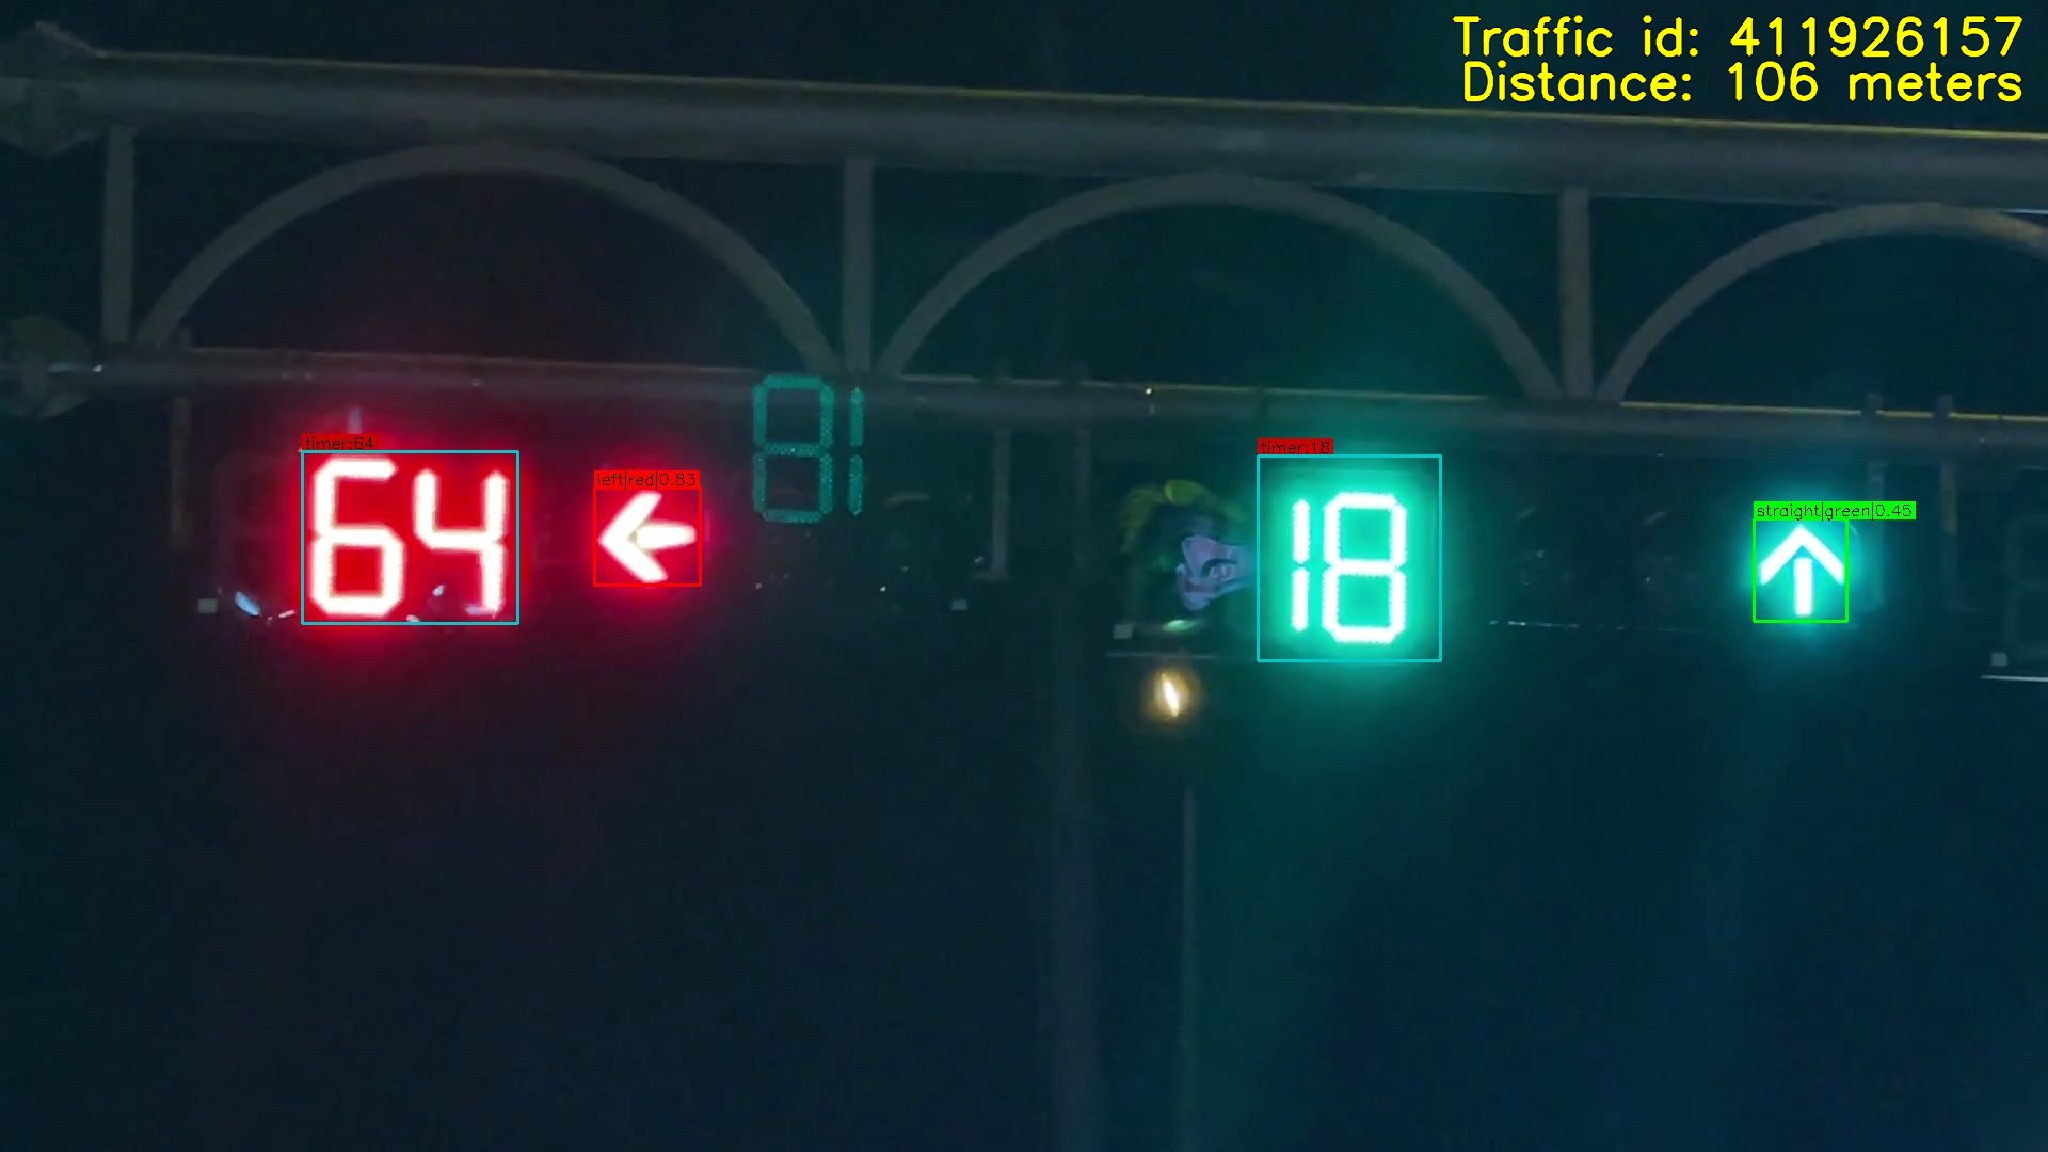
\includegraphics[width=0.75\textwidth]{Images/chapter4/result.png}
%     \vspace{0.5cm}
%     \caption{The result of prototype project}
%     \label{fig:res_project}
% \end{figure}

% Figure~\ref{fig:res_project} illustrates the experimental result obtained from the implemented prototype system. The figure shows the output generated by the ClientSensor application after receiving processed data from the ProviderSensor through the Adaptive AUTOSAR communication mechanism.

% In this experiment, the ClientSensor performs camera-based traffic light detection using the trained YOLO-MobileNet model. Detected traffic lights are highlighted with bounding boxes, and each detection is annotated with the corresponding class label and confidence score, such as red, yellow, and green signal states. The visualization demonstrates that the system is capable of identifying multiple traffic light instances within a single frame and distinguishing different signal colors under indoor test conditions.

% The execution logs displayed in the terminal confirm the end-to-end data flow within the Adaptive AUTOSAR environment. The ProviderSensor successfully publishes processed sensor data, which is then received and consumed by the ClientSensor via SOME/IP with transport protocol (SOME/IP-TP). The logs indicate correct service discovery, data transmission, and event handling between the two applications. Furthermore, the generated output image is stored locally, verifying that the perception results are correctly transferred and processed at the application level.

% Overall, this result validates the functional correctness of the prototype, demonstrating successful integration of deep learning–based perception with Adaptive AUTOSAR service-oriented communication. While the experiment is conducted in a controlled environment and does not represent full automotive deployment conditions, it confirms the feasibility of the proposed architecture and provides a solid foundation for further system optimization and real-world validation.

\subsection{Experimental Setup}
To evaluate the end-to-end functionality of the proposed ADAS architecture followed by the Figure~\ref{fig:archDesign_project}, a hardware-in-the-loop (HIL) experiment was conducted, as previously illustrated in Figure~\ref{fig:hw_arch} in Chapter 2. The setup was designed to simulate a practical in-vehicle network. Specifically, a Raspberry Pi 5 was utilized as the edge computing node to run the Provider application, which handles heavy tasks such as model inference and sensor data collection. A standard USB UVC webcam was connected to capture real-time video streams, while a GPS module supplied accurate vehicle positioning data via a UART interface.
To create a realistic distributed environment, the Client application and the visualization Human-Machine Interface (HMI) were hosted on a separate monitoring computer. This machine was connected to the Raspberry Pi 5 over a Local Area Network (LAN). This separation is important because it ensures that the edge node's processing power is dedicated entirely to AI inference, rather than displaying graphics. 

Furthermore, the overall effectiveness of this setup relies on well-trained perception models. The specific datasets and training configurations used to develop the YOLO26-MobileNetV4 model and the lightweight multi-head CNN timer detector are discussed in detail in Section~\ref{sub:datasetYolo} and Section~\ref{sec:dataCNN}, respectively.

\subsection{System Evaluation}
\begin{figure}[H]
    \centering
    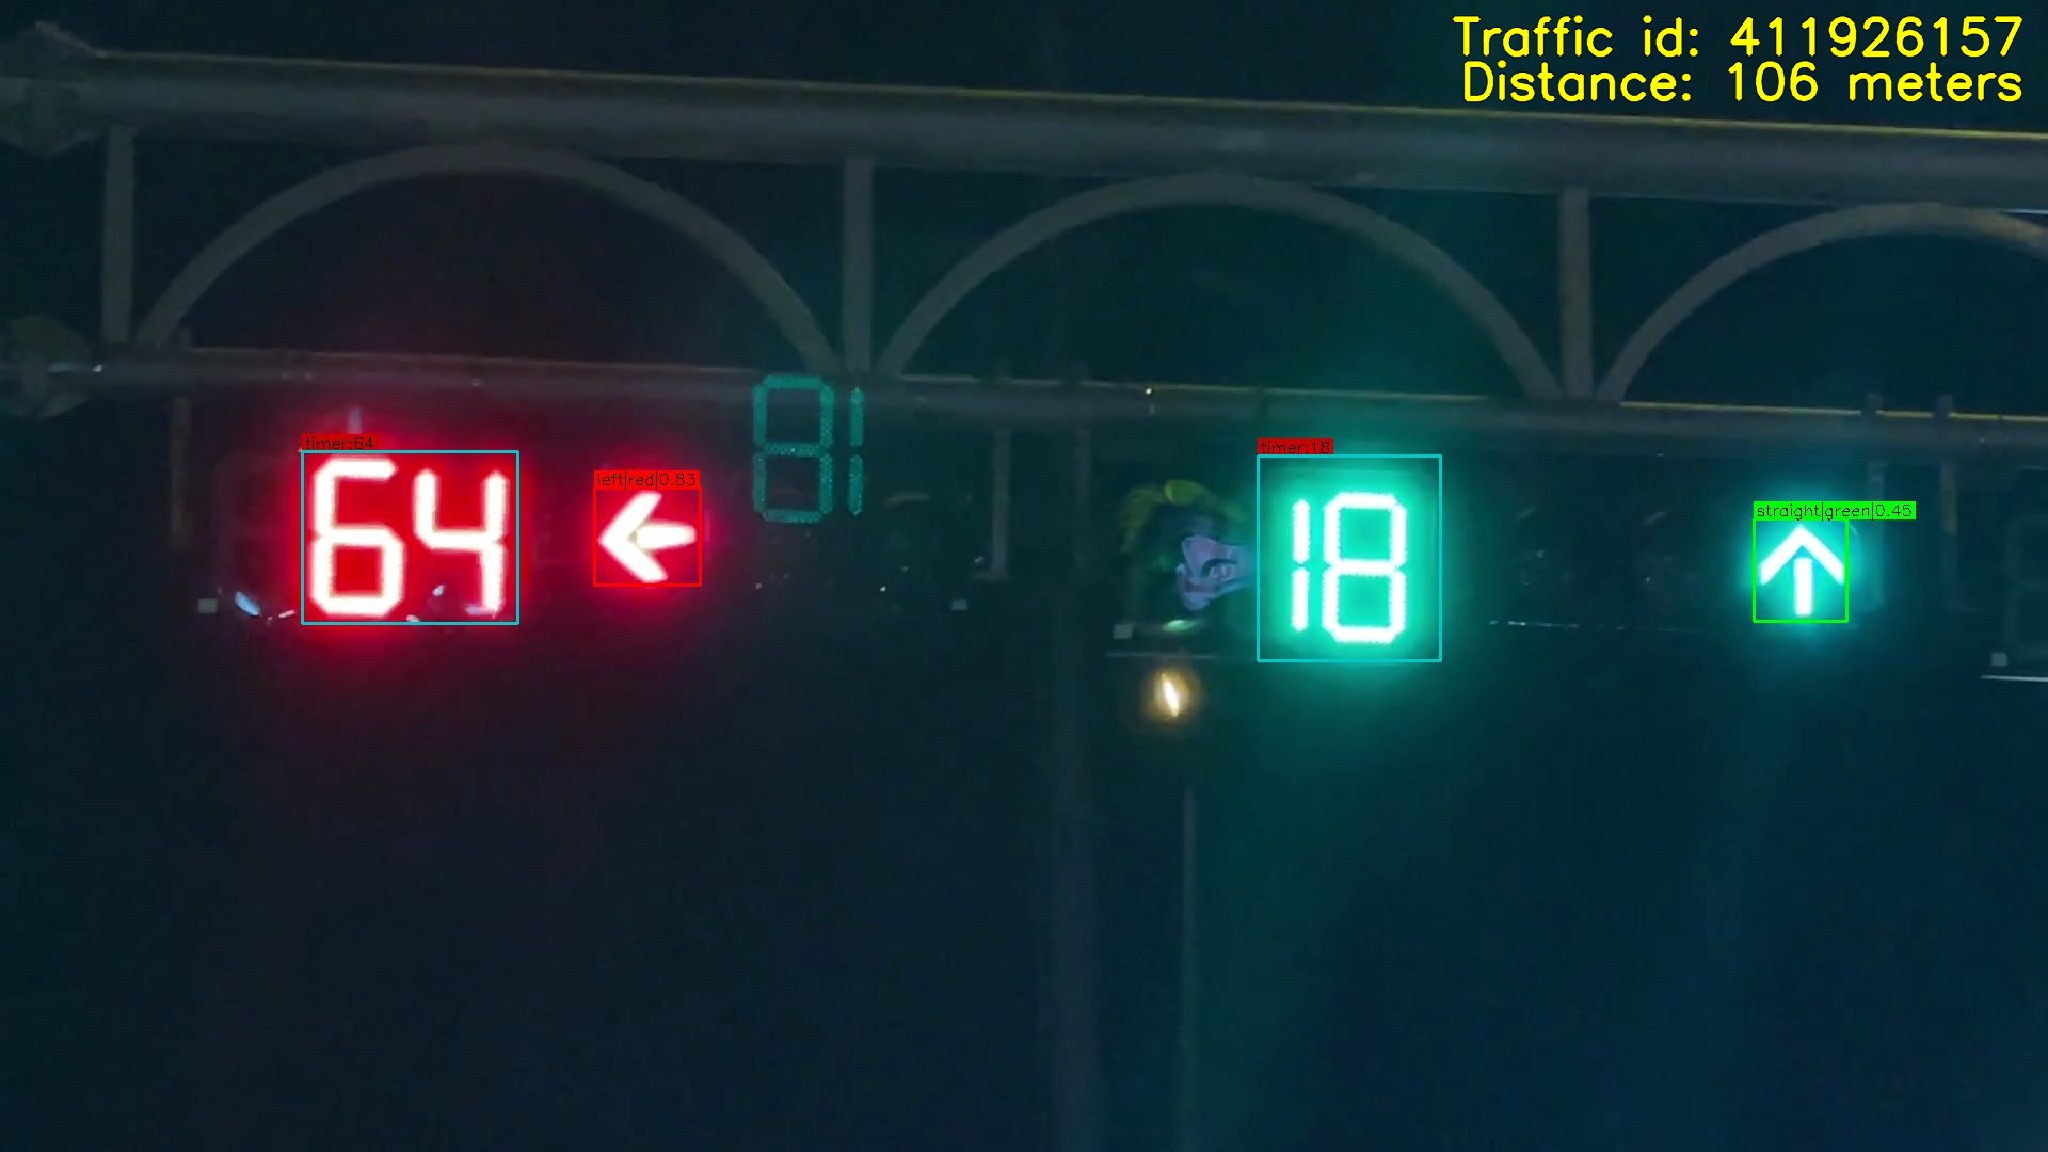
\includegraphics[width=0.75\textwidth]{Images/chapter4/result.png}
    \vspace{0.5cm}
    \caption{Prototype output displayed by the HMI/monitor}
    \label{fig:res_project}
\end{figure}

Figure~\ref{fig:res_project} presents the final visualization produced by the prototype. The monitoring HMI successfully received the data stream from the Client application over the TCP connection. The overlay in the upper-right corner reflects the traffic-light node metadata extracted from the DDS payload, correctly identifying \texttt{Traffic id: 411926157} at a \texttt{Distance: 106 meters}.

During execution, the Provider's perception pipeline successfully captured the camera frame, recognized the traffic light states, and annotated the image. The output highlights a red right-turn signal with a countdown of \texttt{64} seconds and a green straight signal with \texttt{18} seconds remaining. The seamless presentation of both the annotated image and the corresponding GPS metadata confirms that the \texttt{GpsJpegWireHeader} parsing logic functions correctly on the Client side. 

Furthermore, the successful display verifies the reliability of the underlying communication architecture. The \texttt{CycloneDDS-CXX} middleware managed the service discovery and the transportation of the \texttt{imageDataEvent} without observable payload corruption. The experiment demonstrates that the combination of edge-based perception, DDS-driven data distribution, and TCP-based visualization can sustain the required data flow for an ADAS prototype without relying on generic system boilerplates.

With the technical implementations and methodological frameworks thoroughly detailed and validated in Chapter 4, the primary objectives of this research have been addressed. Transitioning into Chapter 5, the focus will shift towards a final synthesis of the project. The upcoming chapter will offer a conclusive summary of the findings, reflect on the practical implications of the developed ADAS system, and propose viable recommendations for future enhancements.


\chapter{Project Prototype}

This chapter presents the implementation of the proposed red-light warning prototype. Inspired by the traffic light recognition approach combining a monocular camera with intelligent transport system data~\cite{Lee2022TrafficLightRecognition}, this prototype utilizes GPS coordinates to calculate the vehicle's distance to the nearest traffic-light node. Upon entering a predefined warning zone, the camera-based perception pipeline is triggered to identify the traffic light direction, classify the signal state, and extract the countdown timer. The processed data is then transmitted to the user display interface.

\begin{figure}[H]
    \centering
    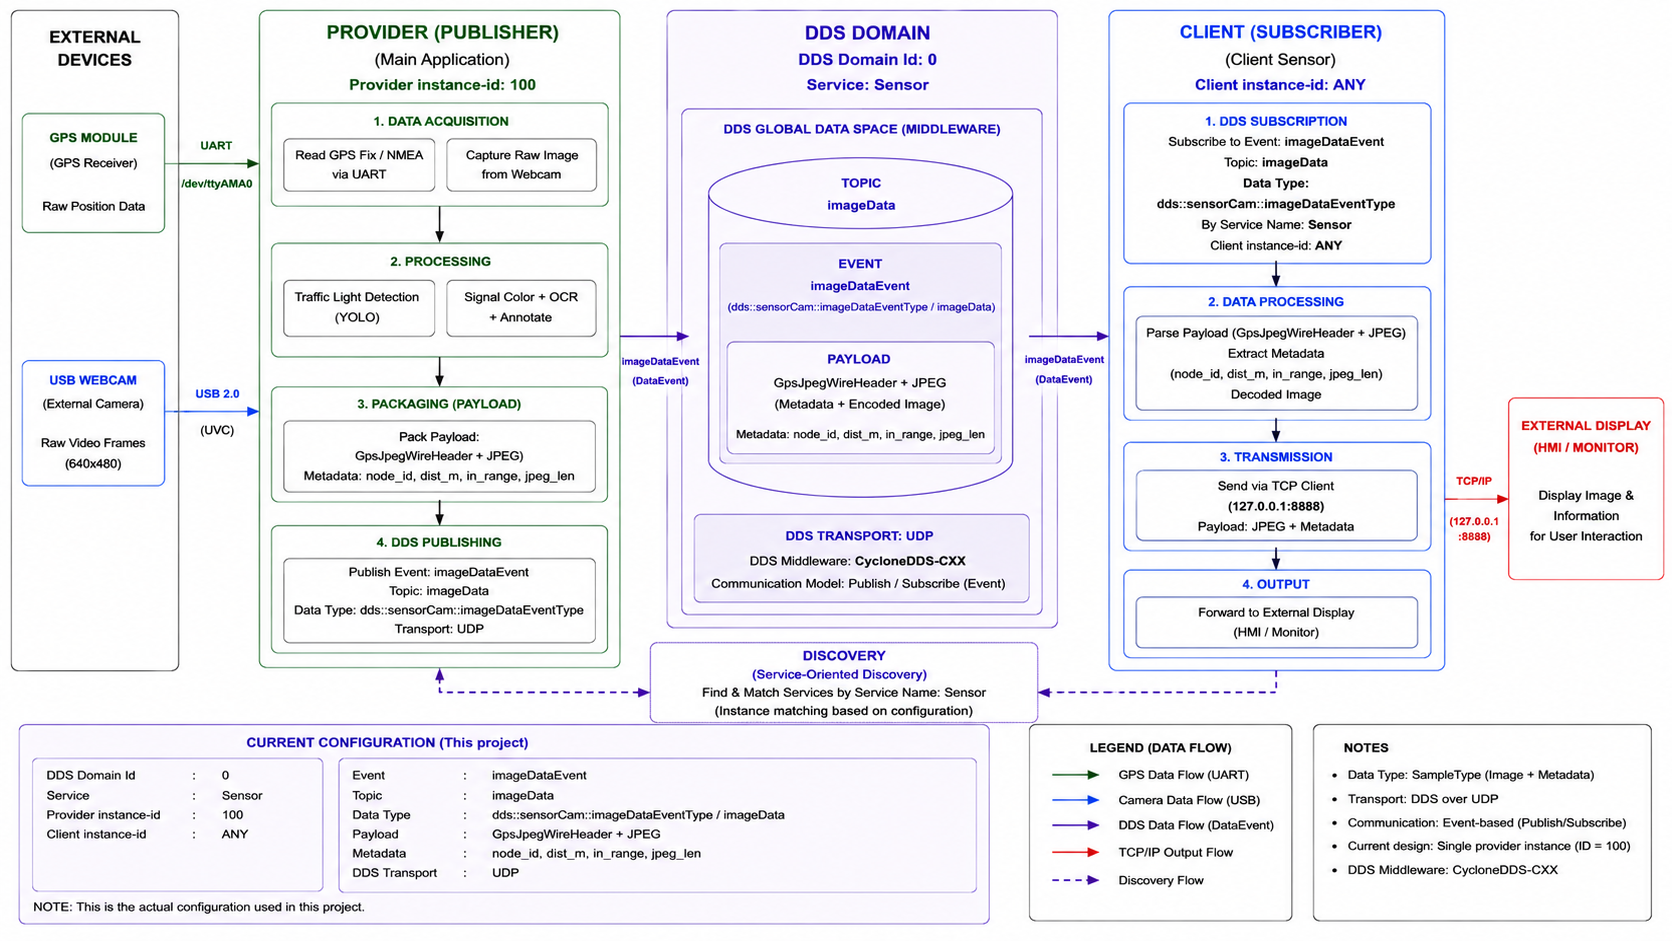
\includegraphics[width=1\textwidth]{Images/chapter4/architecture.png}
    \vspace{0.5cm}
    \caption{The architecture design of prototype project}
    \label{fig:archDesign_project}
\end{figure}

Figure~\ref{fig:archDesign_project} illustrates the architecture of the prototype deployed on a Raspberry Pi 5. The design adopts a service-oriented approach, where functionalities are decoupled into distinct applications communicating via the DDS (Data Distribution Service) middleware (\texttt{CycloneDDS-CXX}).

The architecture comprises two main components:
\begin{itemize}
    \item \textbf{Provider (Main Application):} Handles data acquisition from the GPS module and USB webcam. It executes the deep learning pipeline (YOLO detection, color classification, and OCR), encodes the output into a \texttt{GpsJpegWireHeader} along with JPEG bytes, and publishes the payload as a DDS event.
    \item \textbf{Client (Client Sensor):} Subscribes to the DDS event, parses the payload, and forwards the reconstructed JPEG and metadata over a TCP connection to an external HMI/Monitor for visualization.
\end{itemize}

This separation of concerns allows for independent deployment and testing of perception and visualization tasks. The specific implementation workflows for the Provider and Client are detailed in the following subsections.

\section{Provider Sensor (Publisher)}


% \chapter{Flow Chart}
% \begin{figure}[H]
% \centering
% \begin{tikzpicture}[
%     node distance=1.5cm,
%     every node/.style={font=\small},
%     startstop/.style={
%         rectangle, rounded corners,
%         minimum width=3.6cm,
%         minimum height=0.9cm,
%         draw, align=center
%     },
%     process/.style={
%         rectangle,
%         minimum width=4.4cm,
%         minimum height=0.9cm,
%         draw, align=center
%     },
%     decision/.style={
%         diamond,
%         aspect=2.8,
%         minimum width=2.6cm,
%         minimum height=0.85cm,
%         inner sep=1.5pt,
%         draw, align=center
%     },
%     arrow/.style={->, thick},
% ]

% % ===== Nodes =====
% \node (start) [startstop] {Application Start};

% \node (init) [process, below of=start] {Initialize ProviderSensor};

% \node (tflite) [process, below of=init] {Initialize TFLite Model};

% \node (checkinit) [decision, below of=tflite, yshift=-0.5cm]
% {Initialization Successful};

% \node (terminate) [startstop, right=3.8cm of checkinit]
% {Terminate Application};

% \node (startport) [process, below of=checkinit, yshift=-0.4cm]
% {Start Sensorv2 Port};

% \node (run) [process, below of=startport]
% {Run Application Thread};

% \node (caminit) [process, below of=run]
% {Open Camera Device};

% \node (camcheck) [decision, below of=caminit, yshift=-0.5cm]
% {Camera Opened};

% \node (cont) [startstop, below of=camcheck, yshift=-0.4cm]
% {Enter Main Processing Loop};

% % ===== Arrows =====
% \draw [arrow] (start) -- (init);
% \draw [arrow] (init) -- (tflite);
% \draw [arrow] (tflite) -- (checkinit);

% \draw [arrow] (checkinit) -- node[right]{Yes} (startport);
% \draw [arrow] (checkinit.east) -- node[above]{No} (terminate.west);

% \draw [arrow] (startport) -- (run);
% \draw [arrow] (run) -- (caminit);
% \draw [arrow] (caminit) -- (camcheck);

% \draw [arrow] (camcheck) -- node[right]{Yes} (cont);
% \draw [arrow]
%     (camcheck.east)
%     -| node[near start, above]{No}
%     (terminate.south);

% \end{tikzpicture}
% \vspace{0.5cm}
% \caption{Initialization Flow of the ProviderSensor Adaptive Application}
% \label{fig:providersensor_init}
% \end{figure}

% \begin{figure}[H]
% \centering
% \begin{tikzpicture}[
%     node distance=1.4cm,
%     every node/.style={font=\small},
%     startstop/.style={
%         rectangle, rounded corners,
%         minimum width=3.6cm,
%         minimum height=0.9cm,
%         draw, align=center
%     },
%     process/.style={
%         rectangle,
%         minimum width=4.6cm,
%         minimum height=0.9cm,
%         draw, align=center
%     },
%     decision/.style={
%         diamond,
%         aspect=2.6,
%         minimum width=3.2cm,
%         minimum height=1.0cm,
%         inner sep=1.5pt,
%         draw, align=center
%     },
%     arrow/.style={->, thick}
% ]

% % ===== Nodes =====
% \node (loop) [startstop] {Main Processing Loop};

% \node (capture) [process, below of=loop]
% {Capture Camera Frame};

% \node (frameok) [decision, below of=capture]
% {Frame Valid};

% \node (infer) [process, below of=frameok, yshift=-0.4cm]
% {YOLO TFLite Inference};

% \node (post) [process, below of=infer]
% {Post Processing\\ Confidence Filter and NMS};

% \node (drawbox) [process, below of=post]
% {Draw Bounding Boxes};

% \node (encode) [process, below of=drawbox]
% {Encode Frame to JPEG};

% \node (send) [process, below of=encode]
% {Send Data via Sensorv2 Port};

% \node (sleep) [process, below of=send]
% {Sleep to Control Frame Rate};

% % ===== Arrows =====
% \draw [arrow] (loop) -- (capture);
% \draw [arrow] (capture) -- (frameok);

% % Decision: Frame Valid
% \draw [arrow] (frameok) -- node[right]{Yes} (infer);
% \draw [arrow]
%     (frameok.east) -- ++(2.2cm,0)
%     |- node[near start, above]{No} (capture.east);

% % Main pipeline
% \draw [arrow] (infer) -- (post);
% \draw [arrow] (post) -- (drawbox);
% \draw [arrow] (drawbox) -- (encode);
% \draw [arrow] (encode) -- (send);
% \draw [arrow] (send) -- (sleep);

% % Loop back
% \draw [arrow]
%     (sleep.west) -- ++(-2.6cm,0)
%     |- (loop.west);

% \end{tikzpicture}
% \vspace{0.5cm}
% \caption{Runtime Processing Loop of the ProviderSensor Application}
% \label{fig:providersensor_runtime}
% \end{figure}

% The process begins with the application startup, followed immediately by the initialization of the \texttt{ProviderSensor} component and the TensorFlow Lite (TFLite) model. The system then verifies if the initialization was successful. If the initialization fails, the application terminates immediately. Upon success, the system starts the \texttt{Sensorv2} communication port and launches the application thread. The flow proceeds to open the camera device. A check is performed to confirm if the camera opened successfully; if not, the application terminates. If the camera is successfully accessed, the system transitions into the main processing loop.

% Once inside the main processing loop, the system continuously captures camera frames. For each iteration, it verifies if the captured frame is valid. If the frame is invalid, the loop restarts. If valid, the system performs inference using the YOLO TFLite model, followed by post-processing steps which include applying a confidence filter and Non-Maximum Suppression (NMS) to refine detections. The system then draws bounding boxes around detected objects and encodes the frame into JPEG format. This processed data is sent via the \texttt{Sensorv2} port. Finally, the loop includes a sleep interval to control the frame rate before repeating the process.




% \chapter{Flow Chart}
\begin{figure}[H]
\centering
\begin{tikzpicture}[
    scale=0.9, transform shape,
    node distance=1.5cm,
    every node/.style={font=\small},
    startstop/.style={
        rectangle, rounded corners,
        minimum width=3.6cm,
        minimum height=0.9cm,
        draw, align=center
    },
    process/.style={
        rectangle,
        minimum width=4.4cm,
        minimum height=0.9cm,
        draw, align=center
    },
    io/.style={
        trapezium, trapezium left angle=70, trapezium right angle=110,
        minimum width=4.0cm, minimum height=0.9cm,
        inner xsep=0.5cm,
        draw, align=center
    },
    decision/.style={
        diamond,
        aspect=2.8,
        minimum width=2.6cm,
        minimum height=0.85cm,
        inner sep=1.5pt,
        draw, align=center
    },
    arrow/.style={->, thick},
]

% ===== Nodes =====
\node (start) [startstop] {Application Start};

\node (init) [process, below of=start] {Initialize Provider Application};

\node (caminit) [process, below of=init] {Open UART (GPS) \& USB (Webcam)};

\node (checkinit) [decision, below of=caminit, yshift=-0.5cm]
{Devices Opened?};

\node (terminate) [startstop, right=3.8cm of checkinit]
{Terminate Application};

\node (startdds) [process, below of=checkinit, yshift=-0.4cm]
{Initialize DDS Publisher\\Service: \texttt{Sensor}, ID: \texttt{100}};

\node (loop) [startstop, below of=startdds]
{Main Processing Loop};

\node (capture) [io, below of=loop]
{1. Data Acquisition (GPS \& Frame)};

\node (yolo) [process, below of=capture]
{2a. YOLO Traffic Light Detection};

% Multi-thread fork (One thread per Direction)
\node (fork) [rectangle, fill=black, inner sep=0pt, minimum width=8.5cm, minimum height=0.15cm, below of=yolo, yshift=-0.2cm] {};

\node (t1) [process, minimum width=3.6cm, align=center, below of=fork, xshift=-2.8cm, yshift=-0.4cm]
{\textbf{Thread 1 (e.g., Left)}\\Extract ROI\\HSV Color Pipeline\\Timer Detection};

\node (tn) [process, minimum width=3.6cm, align=center, below of=fork, xshift=2.8cm, yshift=-0.4cm]
{\textbf{Thread 3 (e.g., Straight)}\\Extract ROI\\HSV Color Pipeline\\Timer Detection};

\node (dots) [below of=fork, yshift=-1.9cm] {\Large $\dots$};

% Multi-thread join
\node (join) [rectangle, fill=black, inner sep=0pt, minimum width=8.5cm, minimum height=0.15cm, below of=t1, xshift=2.8cm, yshift=-0.8cm] {};

\node (pack) [process, below of=join, yshift=0.3cm]
{3. Pack \texttt{GpsJpegWireHeader} + JPEG};

\node (publish) [io, below of=pack]
{4. Publish \texttt{imageDataEvent}\\Topic: \texttt{imageData}};

% ===== Arrows =====
\draw [arrow] (start) -- (init);
\draw [arrow] (init) -- (caminit);
\draw [arrow] (caminit) -- (checkinit);

\draw [arrow] (checkinit) -- node[right]{Yes} (startdds);
\draw [arrow] (checkinit.east) -- node[above]{No} (terminate.west);

\draw [arrow] (startdds) -- (loop);
\draw [arrow] (loop) -- (capture);
\draw [arrow] (capture) -- (yolo);

\draw [arrow] (yolo) -- (fork);
\draw [arrow] (t1.north |- fork.south) -- (t1.north);
\draw [arrow] (tn.north |- fork.south) -- (tn.north);

\draw [arrow] (t1.south) -- (t1.south |- join.north);
\draw [arrow] (tn.south) -- (tn.south |- join.north);
\draw [arrow] (join.south) -- (pack.north);

\draw [arrow] (pack) -- (publish);

% Loop back
\draw [arrow]
    (publish.west) -- ++(-3.8cm,0)
    |- (loop.west);

\end{tikzpicture}
\vspace{0.5cm}
\caption{Processing Flow of the Provider Application}
\label{fig:provider_flow}
\end{figure}

The application initiates the Provider component by acquiring access to the necessary external peripherals: the GPS module via UART (\texttt{/dev/ttyAMA0}) and the external webcam via USB 2.0 (UVC). Upon successful hardware initialization, the application establishes the DDS Publisher node configured for the \texttt{Sensor} service (instance-id~\texttt{100}, Domain Id~\texttt{0}) using the \texttt{CycloneDDS-CXX} stack over UDP. Failure at either the hardware or network initialization stage results in an immediate application termination to ensure system safety.

Once the setup is complete, the execution enters the main processing loop where data acquisition and perception tasks operate continuously. The pipeline captures a raw video frame from the webcam simultaneously with the reading of GPS position data. The raw frame is passed to the YOLO-based Traffic Light Detection module to infer initial bounding boxes. To meet real-time constraints, the subsequent processing stages are parallelized. The algorithm selects the highest-confidence bounding box for each distinct traffic light direction (Left, Right, Straight) and dispatches a dedicated worker thread for each direction. The concurrent operations within these threads are detailed in Figure~\ref{fig:thread_flow}.

\begin{figure}[H]
\centering
\begin{tikzpicture}[
    scale=0.9, transform shape,
    node distance=1.4cm,
    every node/.style={font=\small},
    startstop/.style={
        rectangle, rounded corners,
        minimum width=3.6cm,
        minimum height=0.9cm,
        draw, align=center
    },
    process/.style={
        rectangle,
        minimum width=4.8cm,
        minimum height=0.9cm,
        draw, align=center
    },
    decision/.style={
        diamond,
        aspect=2.8,
        minimum width=3.0cm,
        minimum height=1.0cm,
        inner sep=1.5pt,
        draw, align=center
    },
    arrow/.style={->, thick},
]

% Nodes
\node (start) [startstop] {Thread Start (dirWorker)};

\node (extract_tl) [process, below of=start] {Extract Traffic Light ROI\\on Original High-Res Image};

\node (hsv) [process, below of=extract_tl] {HSV Color Classification};

\node (check_timer) [decision, below of=hsv, yshift=-0.5cm] {Timer Boxes\\Detected?};

\node (find_nearest) [process, below of=check_timer, yshift=-0.5cm] {Find Nearest Timer Box\\(Distance Calculation)};

\node (check_nearest) [decision, below of=find_nearest, yshift=-0.5cm] {Valid Timer\\Box Found?};

\node (extract_timer) [process, below of=check_nearest, yshift=-0.5cm] {Extract Timer ROI\\on Original High-Res Image};

\node (ocr) [process, below of=extract_timer] {Lightweight OCR Model\\(Digit Recognition)};

\node (end) [startstop, right=3.5cm of check_nearest] {Return Direction\\Result};

% Arrows
\draw [arrow] (start) -- (extract_tl);
\draw [arrow] (extract_tl) -- (hsv);
\draw [arrow] (hsv) -- (check_timer);

\draw [arrow] (check_timer) -- node[right]{Yes} (find_nearest);
\draw [arrow] (check_timer.east) -| node[near start, above]{No} (end.north);

\draw [arrow] (find_nearest) -- (check_nearest);
\draw [arrow] (check_nearest) -- node[above]{No} (end.west);
\draw [arrow] (check_nearest) -- node[right]{Yes} (extract_timer);

\draw [arrow] (extract_timer) -- (ocr);
\draw [arrow] (ocr.east) -| (end.south);

\end{tikzpicture}
\vspace{0.5cm}
\caption{Parallel Thread Pipeline for each Direction (dirWorker)}
\label{fig:thread_flow}
\end{figure}

Within each direction's worker thread (\texttt{dirWorker}), the pipeline maps the low-resolution YOLO bounding box back to the original high-resolution frame to extract a precise Region of Interest (ROI). This ROI undergoes an HSV color space transformation to robustly classify the current signal state. Concurrently, the thread identifies any timer boxes detected in the main frame. By calculating geometric distances, the algorithm pairs the nearest valid timer box with the corresponding traffic light direction. If a match is found, the timer's ROI is extracted from the high-resolution frame and passed through a lightweight OCR model to recognize the remaining countdown digits.

Upon the completion of all parallel threads, the main thread synchronizes the multi-directional results. The annotated frame is then JPEG-encoded and serialized alongside a 24-byte \texttt{GpsJpegWireHeader}. This custom header encapsulates the metadata, including the magic value, protocol version, \texttt{in\_range} flag, \texttt{node\_id}, \texttt{dist\_m}, and the payload length (\texttt{jpeg\_len}). Finally, the combined byte sequence is written into the \texttt{imageData} payload of the \texttt{dds::sensorCam::imageDataEventType} structure and published over the DDS network to any subscribed clients.

\section{Client Sensor (Subscriber)}
% \chapter{Flow Chart}

% \begin{figure}[H]
% \centering
% \begin{tikzpicture}[
%     node distance=1.4cm,
%     every node/.style={font=\small},
%     startstop/.style={
%         rectangle, rounded corners,
%         minimum width=3.8cm,
%         minimum height=0.9cm,
%         draw, align=center
%     },
%     process/.style={
%         rectangle,
%         minimum width=4.8cm,
%         minimum height=0.9cm,
%         draw, align=center
%     },
%     decision/.style={
%         diamond,
%         aspect=2.6,
%         minimum width=3.6cm,
%         minimum height=1.1cm,
%         inner sep=1.5pt,
%         draw, align=center
%     },
%     arrow/.style={->, thick}
% ]

% % ===== Nodes =====
% \node (start) [startstop] {Application Start};

% \node (init) [process, below of=start]
% {Initialize ClientSensor};

% \node (register) [process, below of=init]
% {Register Sensorv2\\ Event Handler};

% \node (startport) [process, below of=register]
% {Start Sensorv2 Port};

% \node (wait) [process, below of=startport]
% {Wait for Incoming Data Event};

% \node (dataok) [decision, below of=wait]
% {Data Received};

% \node (decode) [process, below of=dataok, yshift=-0.4cm]
% {Decode JPEG Data};

% \node (decodeok) [decision, below of=decode]
% {Decode Successful};

% \node (save) [process, below of=decodeok, yshift=-0.4cm]
% {Save Image to File};

% \node (saveok) [decision, below of=save]
% {Save Successful};

% \node (logerr) [process, right=4.6cm of decodeok]
% {Log Error};

% % ===== Main Flow =====
% \draw [arrow] (start) -- (init);
% \draw [arrow] (init) -- (register);
% \draw [arrow] (register) -- (startport);
% \draw [arrow] (startport) -- (wait);
% \draw [arrow] (wait) -- (dataok);

% % Data received decision
% \draw [arrow] (dataok) -- node[right]{Yes} (decode);
% \draw [arrow] (dataok.west) -- ++(-1cm,0) |- node[near start, above]{No} (wait.west);

% % Decode path
% \draw [arrow] (decode) -- (decodeok);

% \draw [arrow] (decodeok) -- node[right]{Yes} (save);
% \draw [arrow] (decodeok.east) -- node[near start, above]{No} (logerr.west);

% % Save decision
% \draw [arrow] (save) -- (saveok);

% \draw [arrow]
%     (saveok.west)
%     -- ++(-1.6cm,0)
%     |- node[near start, above]{Yes}
%     (wait.west);
    
% \draw [arrow] (saveok.east) -| node[near start, above]{No} (logerr.south);

% % Error loop back
% \draw [arrow] (logerr.north) |- (wait.east);


% \end{tikzpicture}

% \vspace{0.5cm}
% \caption{ClientSensor Data Reception and Processing Flow}
% \label{fig:clientsensor_flow}
% \end{figure}

% Data Reception and Processing Flow The Client Sensor workflow starts with the application launch and the initialization of the \texttt{ClientSensor} unit. The system registers the \texttt{Sensorv2} event handler and starts the \texttt{Sensorv2} port to enable communication. It then enters a standby state to wait for incoming data events. When data is received, the system attempts to decode the incoming JPEG data. A decision block checks if the decoding was successful; if not, an error is logged. If decoding succeeds, the system proceeds to save the image to a file. A final check confirms if the file save was successful. If the save operation fails, an error is logged; otherwise, the data handling for that event is considered complete.


% \subsection{Flow Chart}

\begin{figure}[H]
\centering
\begin{tikzpicture}[
    node distance=1.4cm,
    every node/.style={font=\small},
    startstop/.style={
        rectangle, rounded corners,
        minimum width=3.8cm,
        minimum height=0.9cm,
        draw, align=center
    },
    process/.style={
        rectangle,
        minimum width=4.8cm,
        minimum height=0.9cm,
        draw, align=center
    },
    decision/.style={
        diamond,
        aspect=2.6,
        minimum width=3.6cm,
        minimum height=1.1cm,
        inner sep=1.5pt,
        draw, align=center
    },
    arrow/.style={->, thick}
]

% ===== Nodes =====
\node (start) [startstop] {Application Start};

\node (init) [process, below of=start]
{Initialize Client Application};

\node (sub) [process, below of=init]
{1. Subscribe \texttt{imageDataEvent}\\Topic: \texttt{imageData}};

\node (wait) [process, below of=sub]
{Wait for \texttt{imageDataEvent}};

\node (dataok) [decision, below of=wait]
{Event Received};

\node (parse) [process, below of=dataok, yshift=-0.4cm]
{2. Parse \texttt{GpsJpegWireHeader} + JPEG};

\node (tcp) [process, below of=parse]
{3. TCP Client\\\texttt{127.0.0.1:8888}};

\node (sendok) [decision, below of=tcp, yshift=-0.4cm]
{Transmission Successful};

\node (out) [process, below of=sendok, yshift=-0.4cm]
{4. Output to External Display};

\node (logerr) [process, right=4.6cm of dataok]
{Log Error};

% ===== Main Flow =====
\draw [arrow] (start) -- (init);
\draw [arrow] (init) -- (sub);
\draw [arrow] (sub) -- (wait);
\draw [arrow] (wait) -- (dataok);

% Data received decision
\draw [arrow] (dataok) -- node[right]{Yes} (parse);
\draw [arrow] (dataok.west) -- ++(-1cm,0) |- node[near start, above]{No} (wait.west);

% Decode path
\draw [arrow] (parse) -- (tcp);
\draw [arrow] (tcp) -- (sendok);

\draw [arrow] (sendok) -- node[right]{Yes} (out);
\draw [arrow] (sendok.east) -| node[near start, above]{No} (logerr.south);

% Loop back
\draw [arrow]
    (out.west)
    -- ++(-1.6cm,0)
    |-
    (wait.west);
    
% Error loop back
\draw [arrow] (logerr.north) |- (wait.east);

\end{tikzpicture}

\vspace{0.5cm}
\caption{Client Data Reception and Processing Flow}
\label{fig:client_flow}
\end{figure}

Upon startup, the Client application initializes its DDS Subscriber node. It registers a listener for the \texttt{imageDataEvent} on the \texttt{imageData} topic, targeting the \texttt{Sensor} service. The application is configured to discover any available provider (instance-id~\texttt{ANY}) operating on Domain Id~\texttt{0}. Once the DDS entities are established via the \texttt{CycloneDDS-CXX} middleware, the subscriber thread blocks and waits for incoming \texttt{dds::sensorCam::imageDataEventType} messages.

Upon receiving an event, the application extracts the \texttt{imageData} payload and decodes its byte structure. The parser reads the initial 24 bytes to reconstruct the \texttt{GpsJpegWireHeader}, extracting vital metadata such as the \texttt{in\_range} flag, \texttt{node\_id}, \texttt{dist\_m}, and \texttt{jpeg\_len}. Subsequently, it extracts the JPEG image bytes corresponding to the \texttt{jpeg\_len} field. 

To bridge the DDS middleware with the user-facing interface, the Client acts as a TCP proxy. It marshals the decoded data into a custom TCP packet structured as \texttt{[uint32 frame\_len][JPEG][uint8 in\_range][int64 node\_id][int32 dist\_m]} and transmits it to the external display monitor listening at \texttt{127.0.0.1:8888}. In case of a socket error, the application logs the failure and attempts reconnection. Otherwise, the HMI updates the visualization with the latest camera frame and GPS metadata, and the subscriber returns to its listening state for the next DDS event.

\section{Experimental Setup and Results}
% \begin{figure}[H]
%     \centering
%     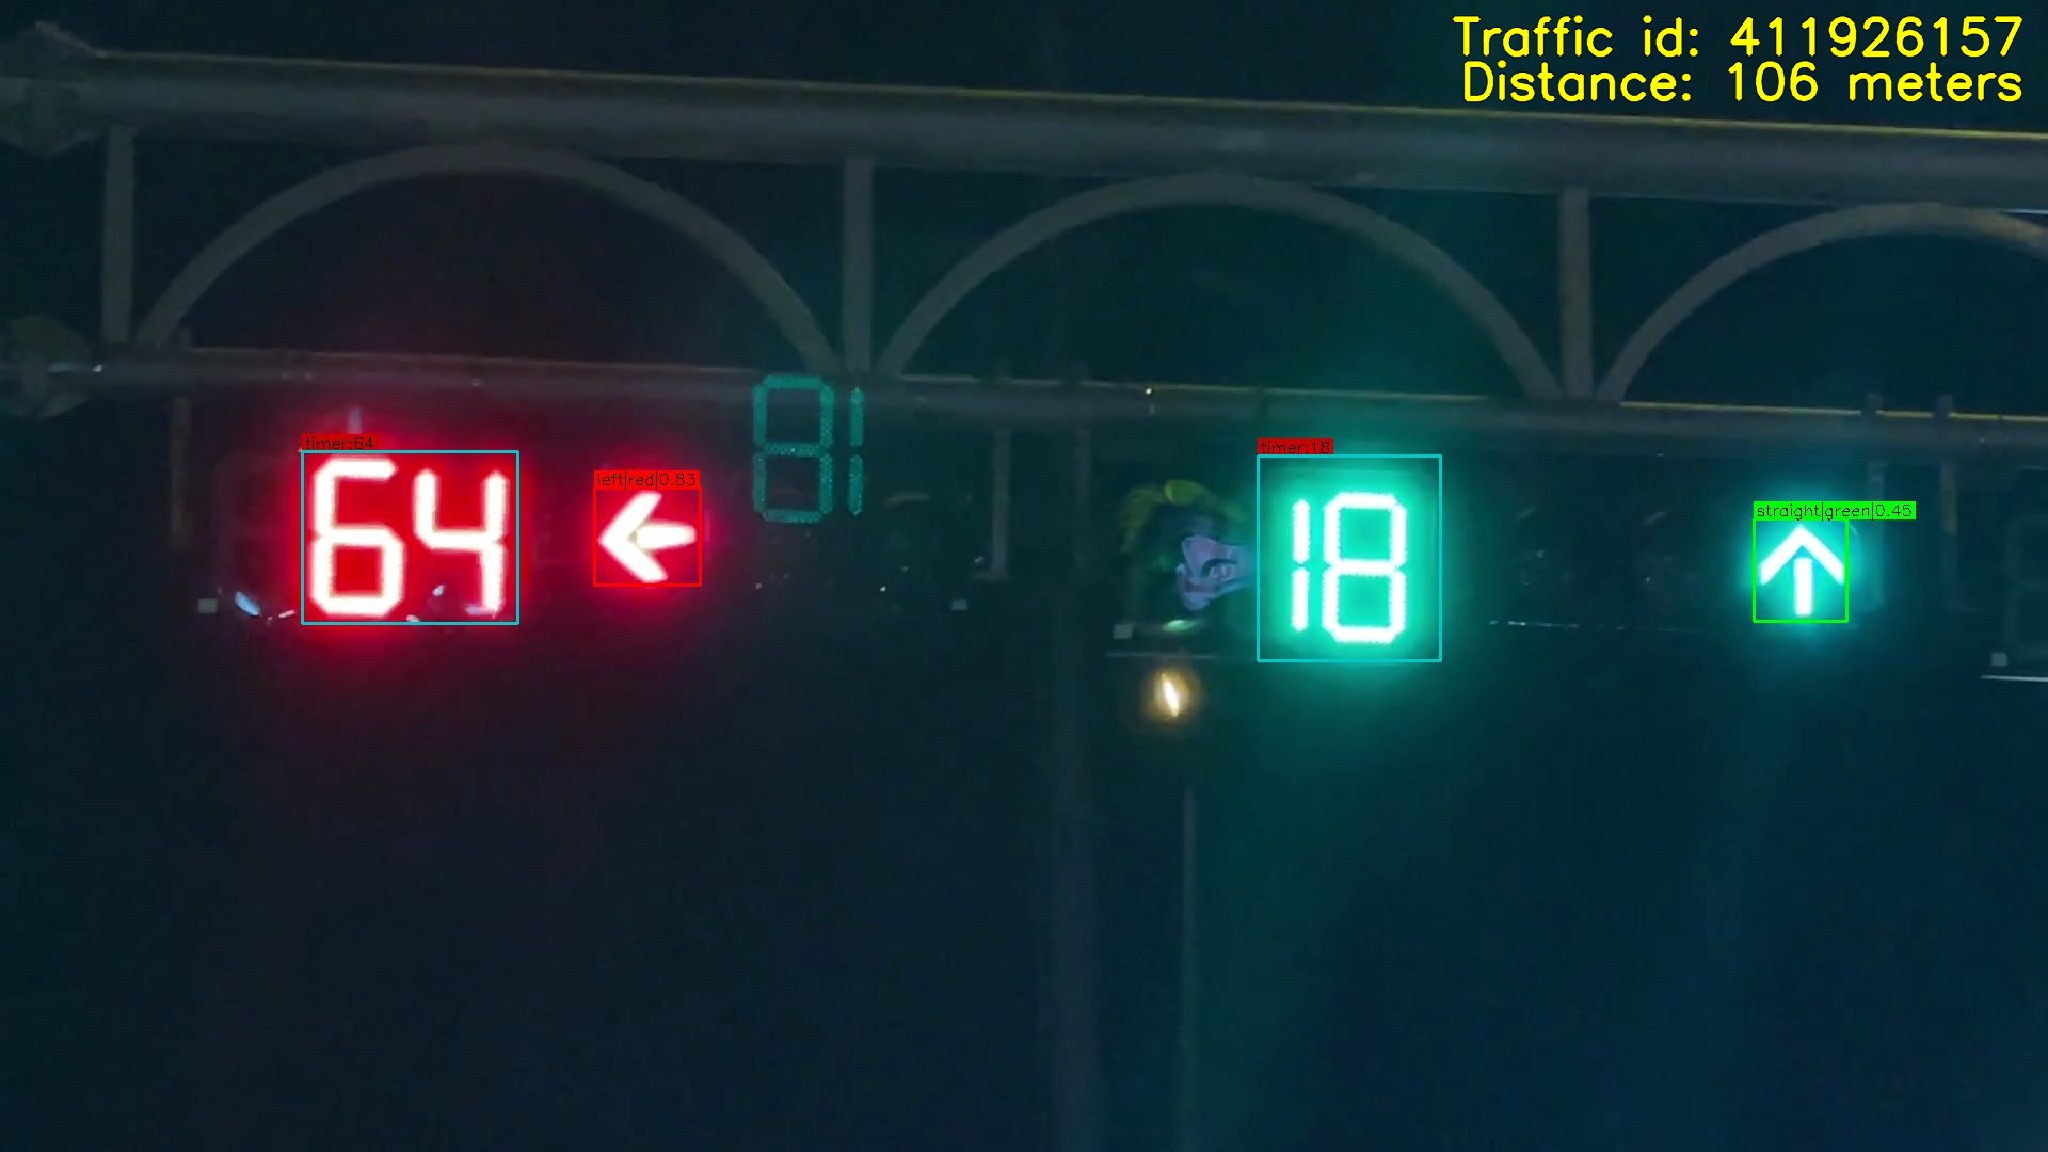
\includegraphics[width=0.75\textwidth]{Images/chapter4/result.png}
%     \vspace{0.5cm}
%     \caption{The result of prototype project}
%     \label{fig:res_project}
% \end{figure}

% Figure~\ref{fig:res_project} illustrates the experimental result obtained from the implemented prototype system. The figure shows the output generated by the ClientSensor application after receiving processed data from the ProviderSensor through the Adaptive AUTOSAR communication mechanism.

% In this experiment, the ClientSensor performs camera-based traffic light detection using the trained YOLO-MobileNet model. Detected traffic lights are highlighted with bounding boxes, and each detection is annotated with the corresponding class label and confidence score, such as red, yellow, and green signal states. The visualization demonstrates that the system is capable of identifying multiple traffic light instances within a single frame and distinguishing different signal colors under indoor test conditions.

% The execution logs displayed in the terminal confirm the end-to-end data flow within the Adaptive AUTOSAR environment. The ProviderSensor successfully publishes processed sensor data, which is then received and consumed by the ClientSensor via SOME/IP with transport protocol (SOME/IP-TP). The logs indicate correct service discovery, data transmission, and event handling between the two applications. Furthermore, the generated output image is stored locally, verifying that the perception results are correctly transferred and processed at the application level.

% Overall, this result validates the functional correctness of the prototype, demonstrating successful integration of deep learning–based perception with Adaptive AUTOSAR service-oriented communication. While the experiment is conducted in a controlled environment and does not represent full automotive deployment conditions, it confirms the feasibility of the proposed architecture and provides a solid foundation for further system optimization and real-world validation.

\subsection{Experimental Setup}
To evaluate the end-to-end functionality of the proposed ADAS architecture followed by the Figure~\ref{fig:archDesign_project}, a hardware-in-the-loop (HIL) experiment was conducted, as previously illustrated in Figure~\ref{fig:hw_arch} in Chapter 2. The setup was designed to simulate a practical in-vehicle network. Specifically, a Raspberry Pi 5 was utilized as the edge computing node to run the Provider application, which handles heavy tasks such as model inference and sensor data collection. A standard USB UVC webcam was connected to capture real-time video streams, while a GPS module supplied accurate vehicle positioning data via a UART interface.
To create a realistic distributed environment, the Client application and the visualization Human-Machine Interface (HMI) were hosted on a separate monitoring computer. This machine was connected to the Raspberry Pi 5 over a Local Area Network (LAN). This separation is important because it ensures that the edge node's processing power is dedicated entirely to AI inference, rather than displaying graphics. 

Furthermore, the overall effectiveness of this setup relies on well-trained perception models. The specific datasets and training configurations used to develop the YOLO26-MobileNetV4 model and the lightweight multi-head CNN timer detector are discussed in detail in Section~\ref{sub:datasetYolo} and Section~\ref{sec:dataCNN}, respectively.

\subsection{System Evaluation}
\begin{figure}[H]
    \centering
    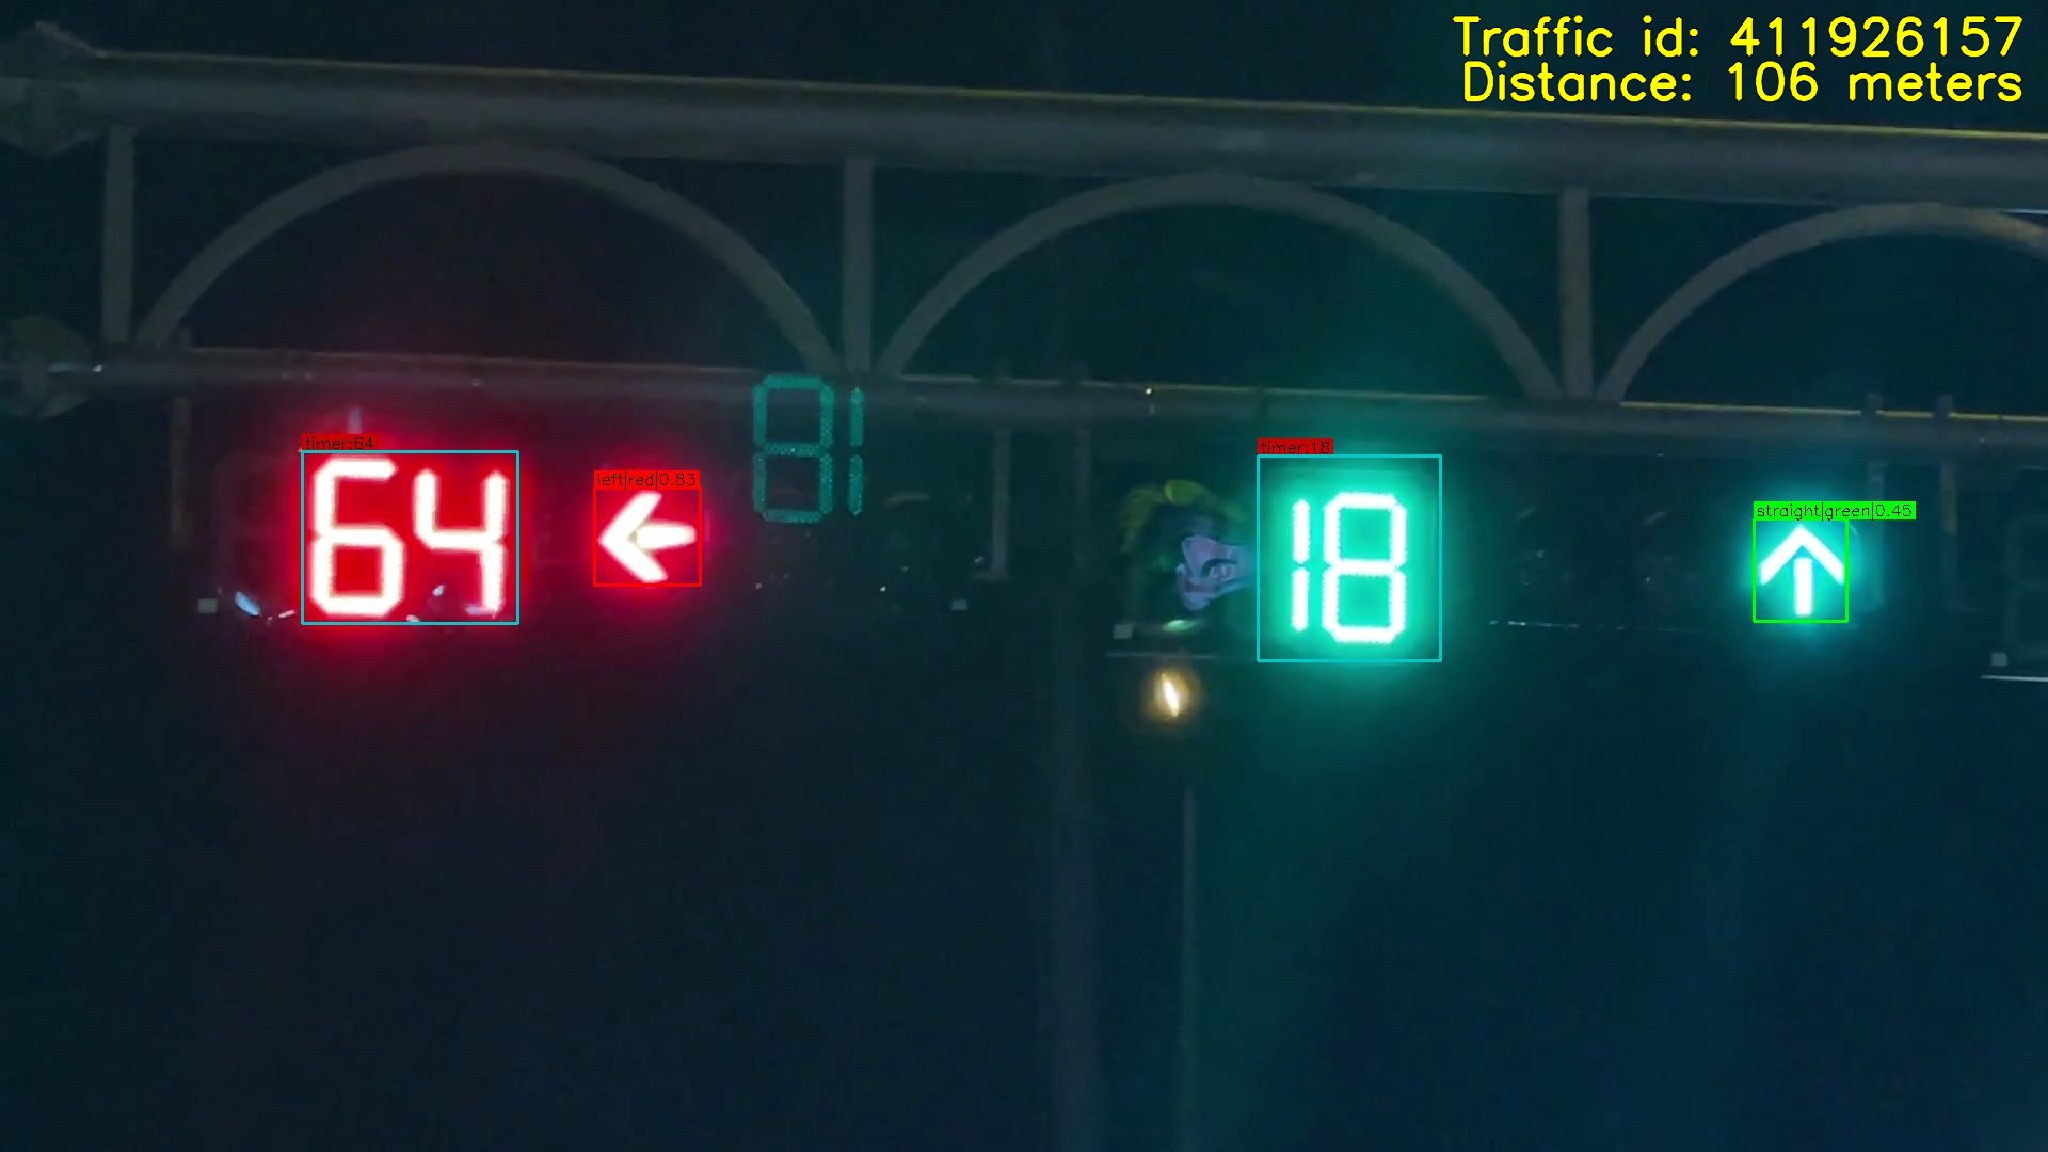
\includegraphics[width=0.75\textwidth]{Images/chapter4/result.png}
    \vspace{0.5cm}
    \caption{Prototype output displayed by the HMI/monitor}
    \label{fig:res_project}
\end{figure}

Figure~\ref{fig:res_project} presents the final visualization produced by the prototype. The monitoring HMI successfully received the data stream from the Client application over the TCP connection. The overlay in the upper-right corner reflects the traffic-light node metadata extracted from the DDS payload, correctly identifying \texttt{Traffic id: 411926157} at a \texttt{Distance: 106 meters}.

During execution, the Provider's perception pipeline successfully captured the camera frame, recognized the traffic light states, and annotated the image. The output highlights a red right-turn signal with a countdown of \texttt{64} seconds and a green straight signal with \texttt{18} seconds remaining. The seamless presentation of both the annotated image and the corresponding GPS metadata confirms that the \texttt{GpsJpegWireHeader} parsing logic functions correctly on the Client side. 

Furthermore, the successful display verifies the reliability of the underlying communication architecture. The \texttt{CycloneDDS-CXX} middleware managed the service discovery and the transportation of the \texttt{imageDataEvent} without observable payload corruption. The experiment demonstrates that the combination of edge-based perception, DDS-driven data distribution, and TCP-based visualization can sustain the required data flow for an ADAS prototype without relying on generic system boilerplates.

With the technical implementations and methodological frameworks thoroughly detailed and validated in Chapter 4, the primary objectives of this research have been addressed. Transitioning into Chapter 5, the focus will shift towards a final synthesis of the project. The upcoming chapter will offer a conclusive summary of the findings, reflect on the practical implications of the developed ADAS system, and propose viable recommendations for future enhancements.